%!TEX root = ../dissertation.tex

\chapter{Evaluation}
\label{chapter:evaluation}




\section{GD capability}
The goal of our work was to bring \gls{gd} to the web browser so it can be used anywhere more easily.
To do this, we implemented a set of primitives that produce several 3D concepts to be used as building blocks for modeling.

Now comes the time to test the environment's ability to be used for \gls{gd}, more specifically to produce diverse 3D models.
In order to evaluate this, we developed several programs that reproduce examples that were previously done in other \gls{gd} environments.
The results of these programs are shown in Figure~\ref{fig:all:examples}.

\begin{figure}
  \centering
  \begin{subfigure}[b]{0.25\linewidth}
    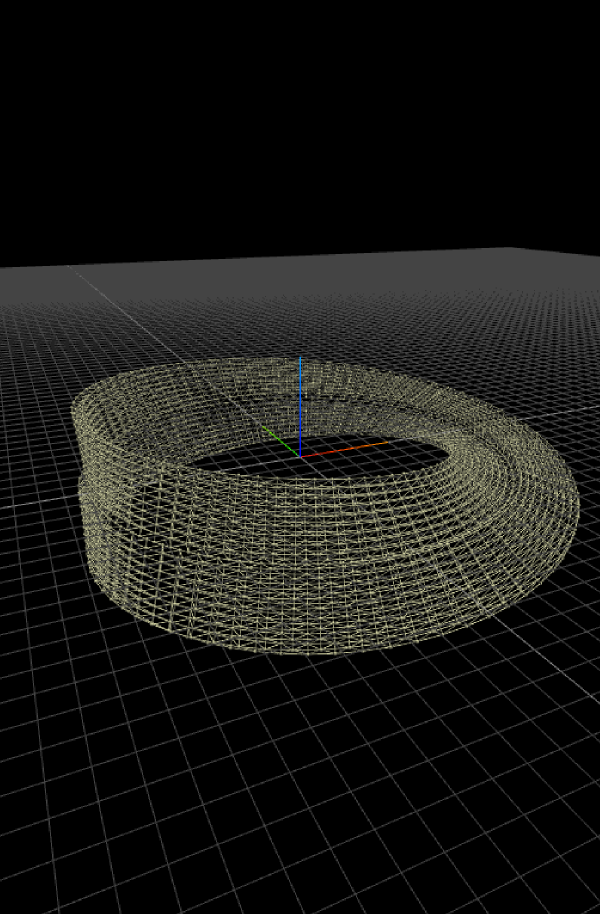
\includegraphics[width=1.0\linewidth]{./images/all_examples/trelica_mobius_crop}
    \caption{Mobius Truss}
    \label{fig:ex:mobius}
  \end{subfigure}
  \begin{subfigure}[b]{0.25\linewidth}
    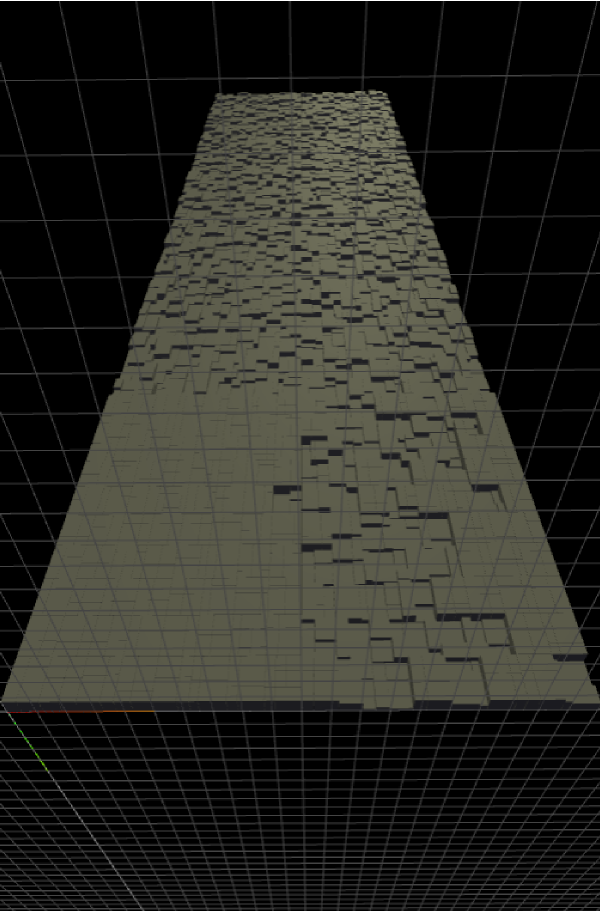
\includegraphics[width=1.0\linewidth]{./images/all_examples/sheung_wan_hotel_crop}
    \caption{Sheung-Wan Hotel}
    \label{fig:ex:sheung:wan}
  \end{subfigure}
  \begin{subfigure}[b]{0.25\linewidth}
    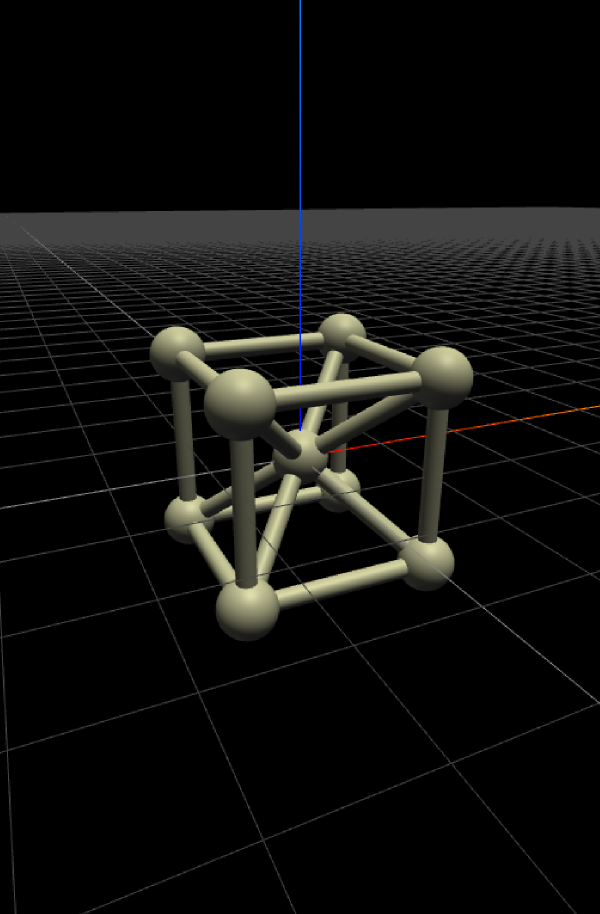
\includegraphics[width=1.0\linewidth]{./images/all_examples/atomium_crop}
    \caption{Atomium}
    \label{fig:ex:atomium}
  \end{subfigure}
  \begin{subfigure}[b]{0.25\linewidth}
    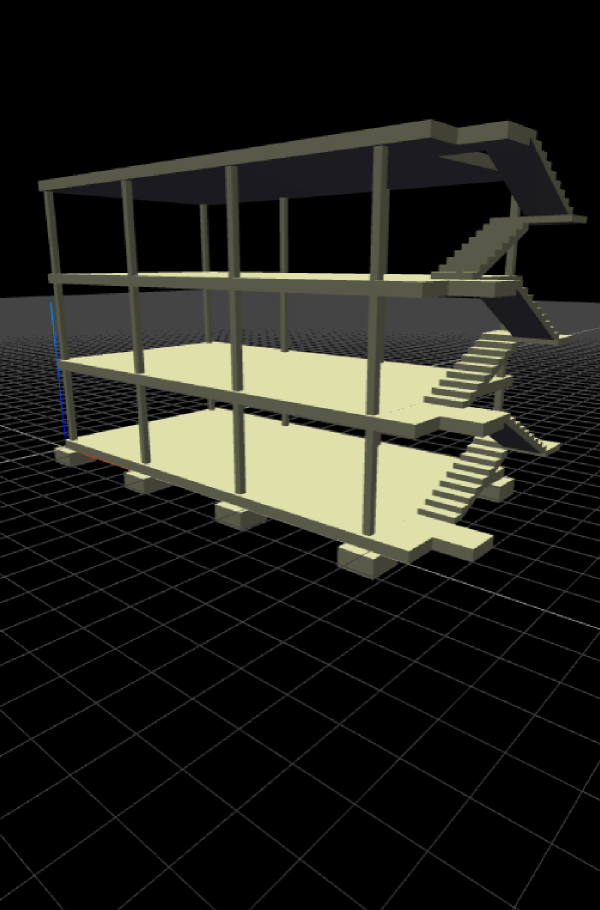
\includegraphics[width=1.0\linewidth]{./images/all_examples/dom_ino_crop}
    \caption{Dom-ino}
    \label{fig:ex:domino}
  \end{subfigure}
  \begin{subfigure}[b]{0.25\linewidth}
    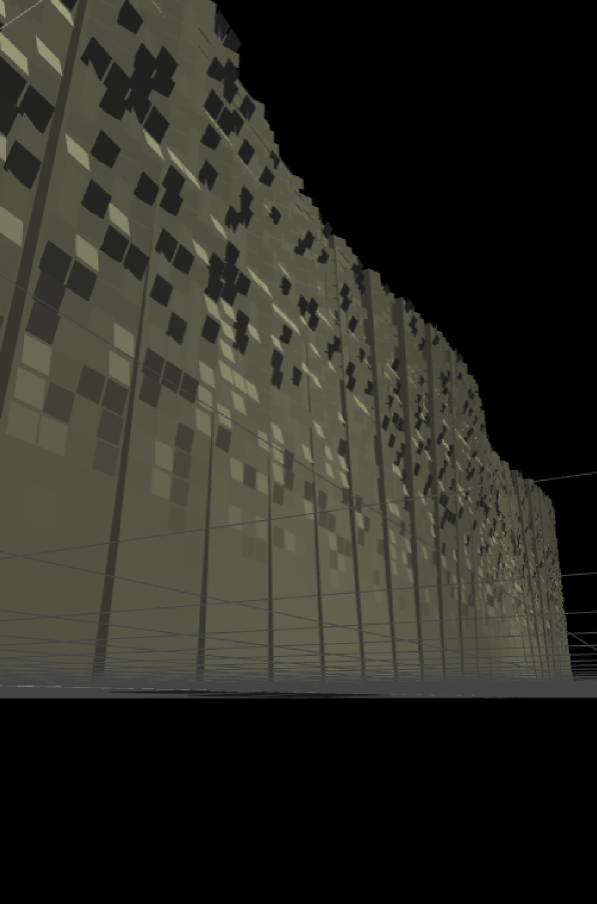
\includegraphics[width=1.0\linewidth]{./images/all_examples/nolan_facade_crop}
    \caption{Nolan Facade}
    \label{fig:ex:nolan}
  \end{subfigure}
  \begin{subfigure}[b]{0.25\linewidth}
    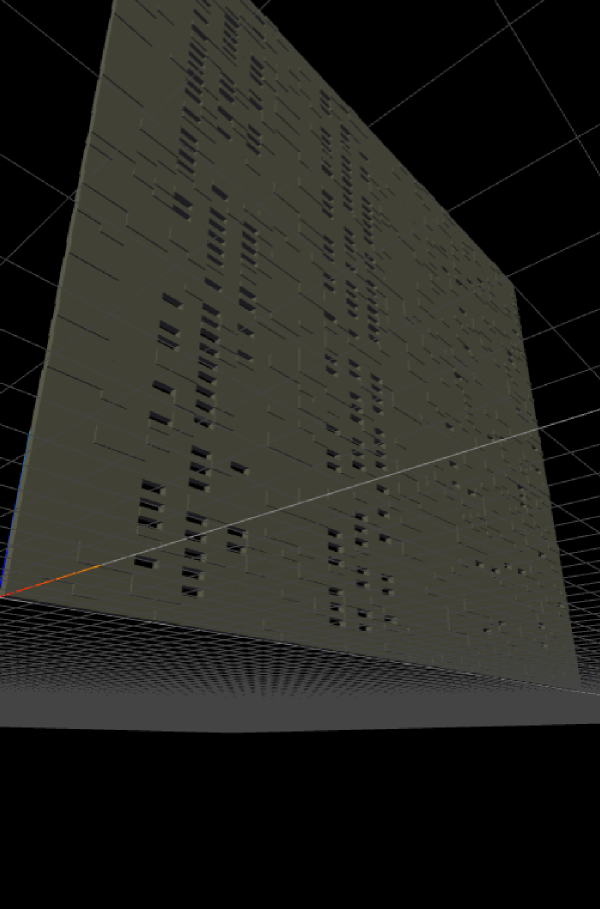
\includegraphics[width=1.0\linewidth]{./images/all_examples/ines_wall_crop}
    \caption{Ines Wall}
    \label{fig:ex:ines:wall}
  \end{subfigure}
  \begin{subfigure}[b]{0.25\linewidth}
    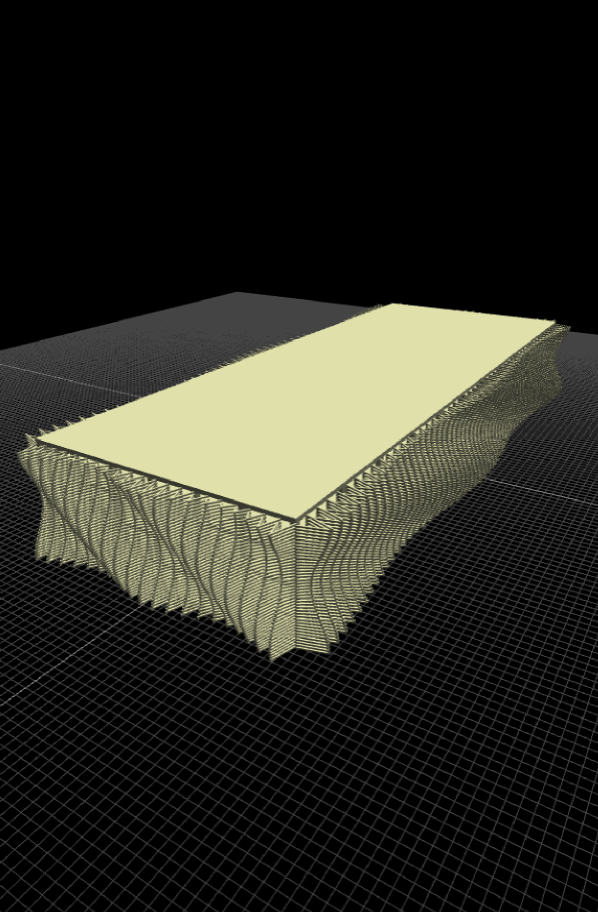
\includegraphics[width=1.0\linewidth]{./images/all_examples/edificio_carmo_crop}
    \caption{Carmo Facade}
    \label{fig:ex:carmo:facade}
  \end{subfigure}

  %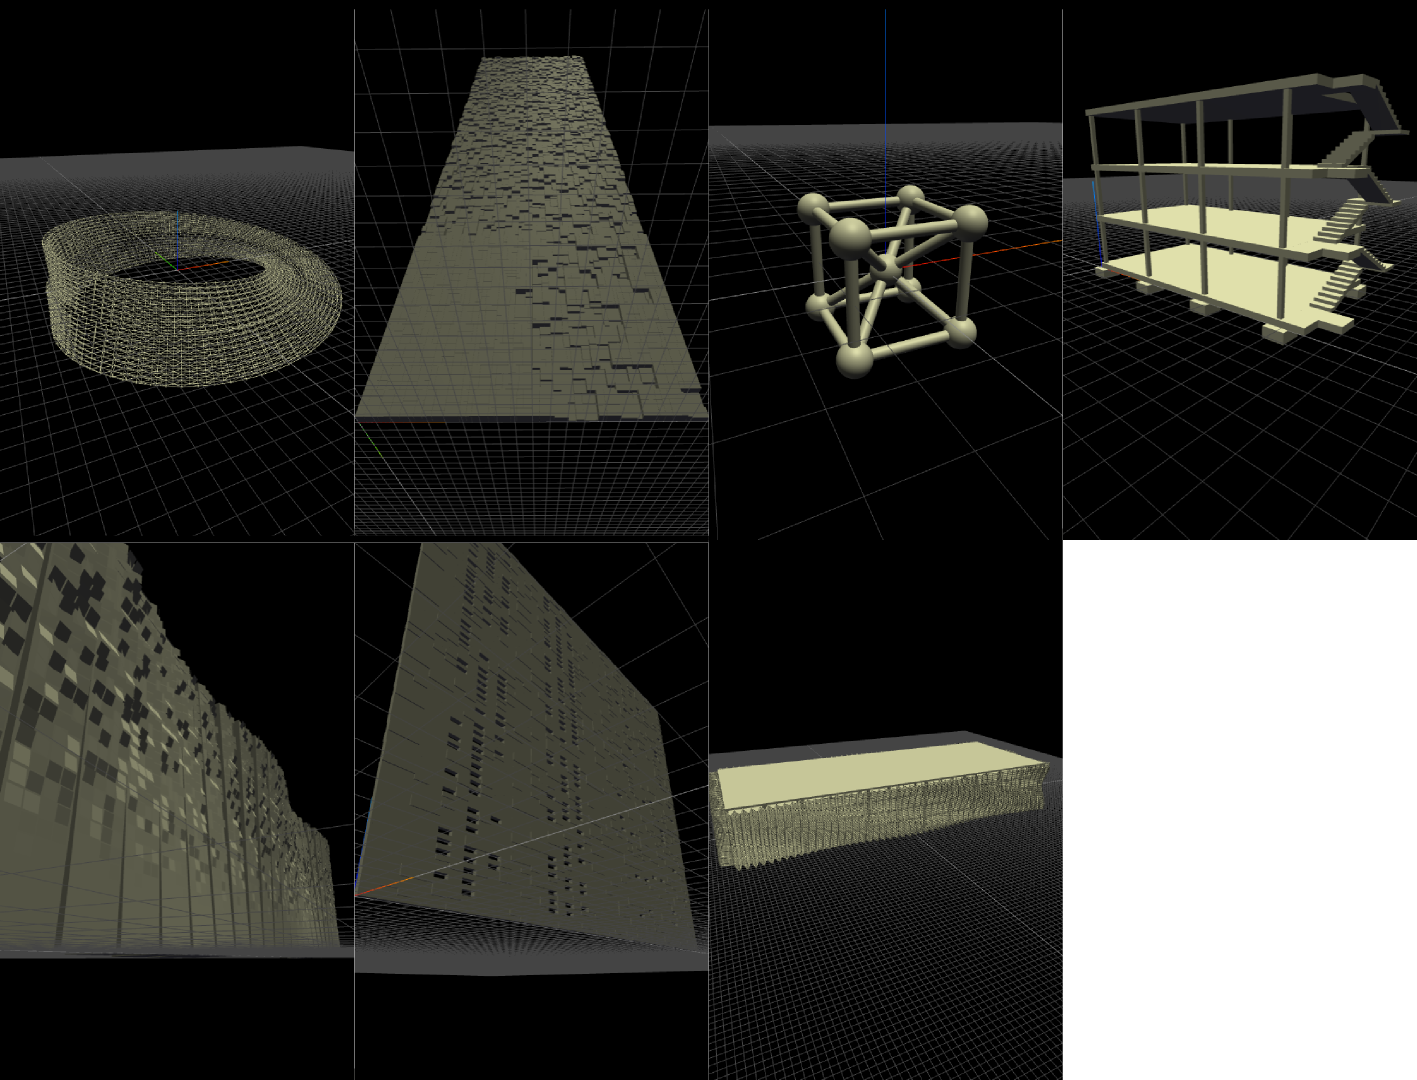
\includegraphics[width=12cm]{./images/all_examples}
  \caption{Renderings of results of the implemented example programs.}
  \label{fig:all:examples}
\end{figure}

As shown, the environment can produce interesting results with varying degrees of complexity.
The range of results is still limited by the primitives currently implemented.
None of these examples make use of \gls{csg} operations like union, intersection and difference as these were not implemented.
Nevertheless, it is possible to add support for these since there are already JavaScript implementations of \gls{csg}, like the case of OpenJSCAD's.


%\section{Real Use}
%{\it This is where I give the prototype to an architect, ask him to do a building, get his feedback, and tell it to the world.}


\section{Performance}
There are several areas where performance plays an important part when using the environment.

To evaluate our solution's performance, we have tested several situations: (1) we compared program running times in the web page with running times of the same programs in Rosetta; (2) we compared program running times with export times; (3) we compared how traceability data collection affects program running times; and (4) we compared export times with times from running programs directly in Rosetta.

\paragraph{Setup}
All tests were performed on a computer with an Intel Core i7-3630QM CPU, 16GB DDR3 RAM and an AMD Radeon HD 7970M GPU.

The web page and the remote CAD service were hosted at the same computer.

%The source code of each program used in the tests can be found in Appendix~\ref{appendix:test:source:code}. %{\bf(either here, appendix or github)}

\begin{figure}
  \centering
  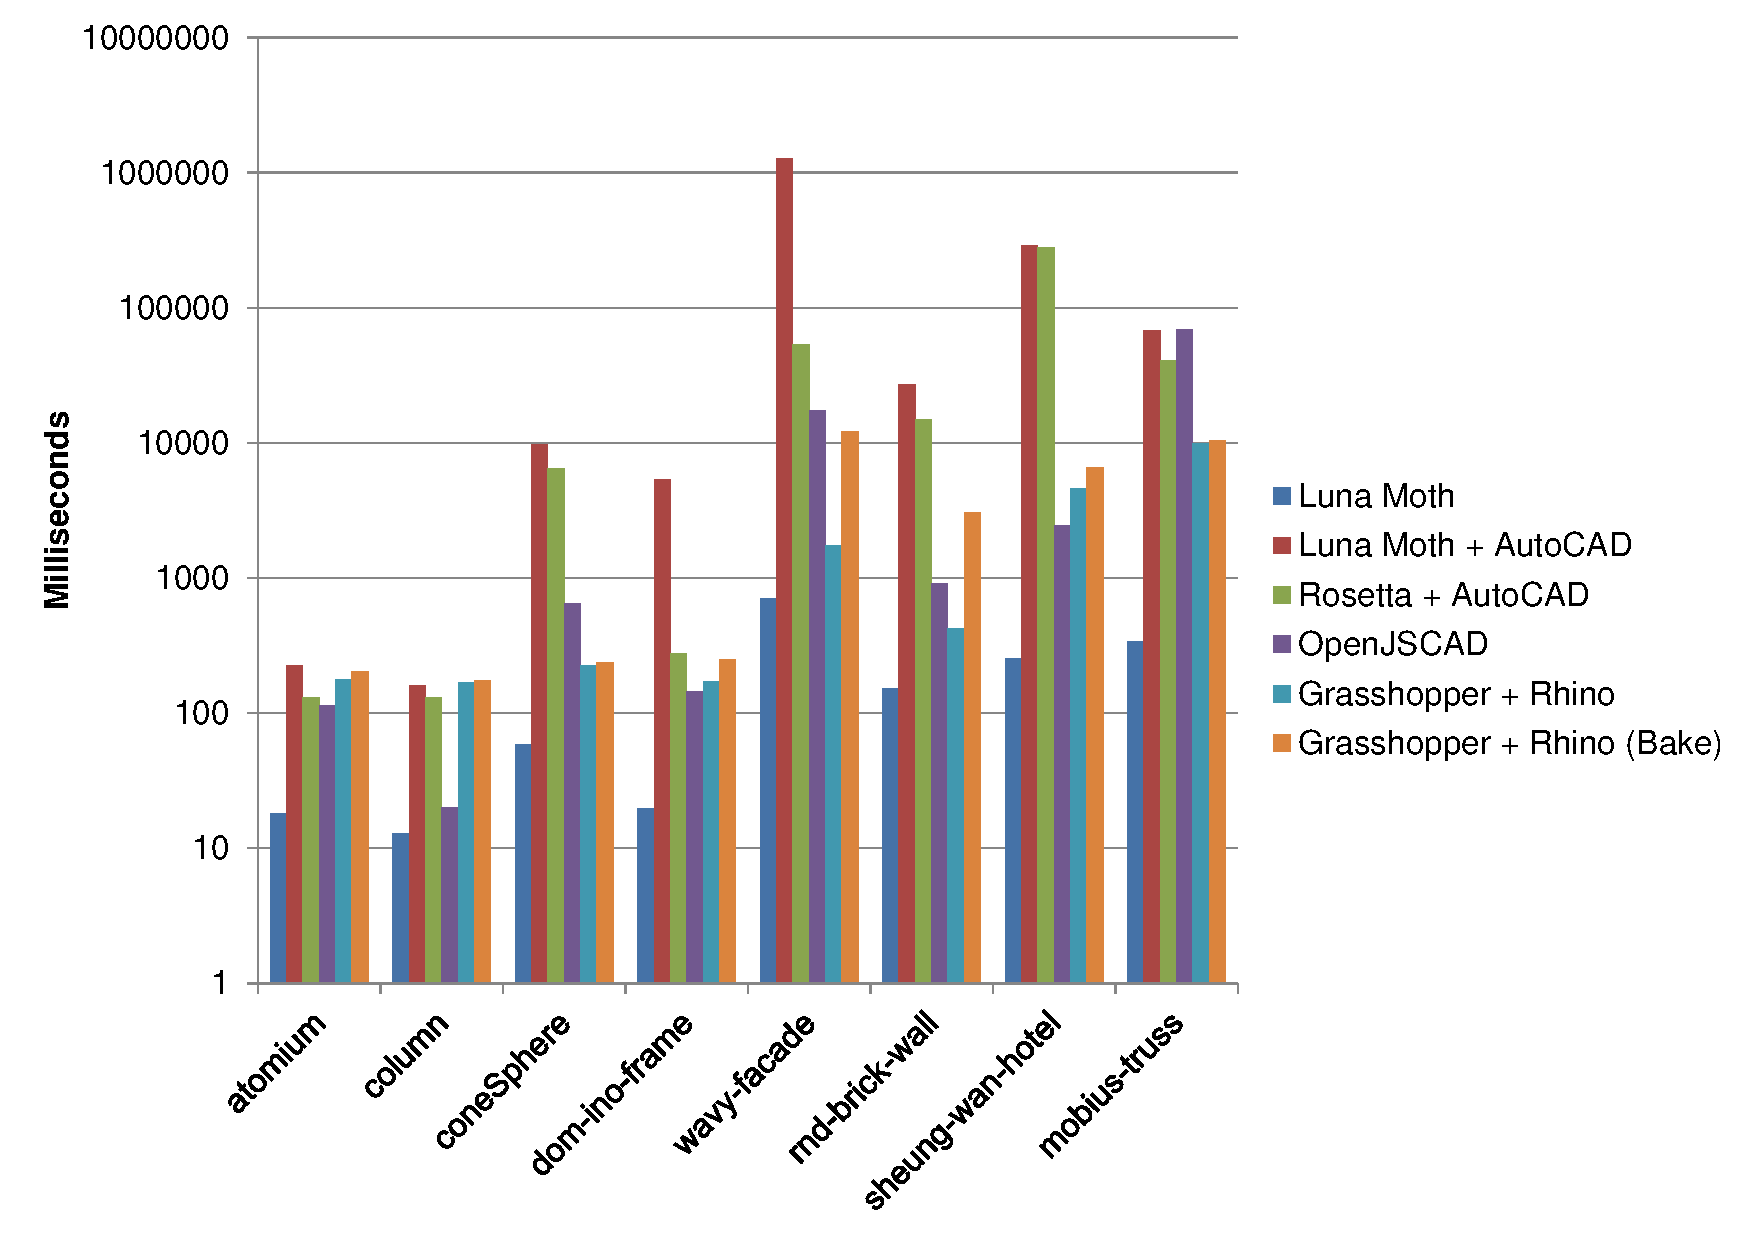
\includegraphics[width=12cm]{./images/run_export_rosetta_times}
  \caption{Comparison of running times for the web, the export process and Rosetta.}
  \label{fig:run:export:rosetta:chart}
\end{figure}



\subsection{Running Performance}
Running performance is a prevalent part of programming in \gls{gd} since it dictates the complexity of the programs that can be explored interactively.
After a program as become too complex, hence too slow, it can no longer be tested as a whole.
So, it needs to be split into smaller parts that are still fast enough to be explored interactively.

To see how the performance of our web-based \gls{gd} environment compares to the existing environments, we compared the time each takes to generate identical models.
First, we implemented a version of the program using each environment's programming language and, then, measured the time each took to complete.
The times can be seen in Figure~\ref{fig:run:export:rosetta:chart}.
Times are the average of three runs.

As can be seen, the relationship between running times varies from program to program, although the web page is consistently faster than Rosetta connected to AutoCAD.
More specifically, Rosetta's running times for both the Mobius and Ines Wall programs are around 40x the running times on the web page.
% and around 500x for the Sheung-Wan Hotel program.

With this in mind, we can say that our solution can provide better feedback than Rosetta.

%We compared our environment with Rosetta (using the OpenGL backend), OpenJSCAD and Rhino+Grasshopper.


\subsection{Export Performance}
When time comes to pass on the building design to other people that use different tools --- like mechanical, electric, plumbing services or even other architects --- the architect must provide it in a format compatible with their tools.
This has been covered in our solution by letting the program that generates the building model run in a \gls{cad} tool.

The next step was to evaluate how the execution time differs between the normal running process and the remote \gls{cad} running process.
To measure the difference, we ran two example programs using both processes and measured the time each took to complete.
The chart in Figure~\ref{fig:run:export:rosetta:chart} shows the running times of two programs for each process.
Times are the average of three runs.

As seen in the chart, comparing export times to normal running times, export times are around 200x the normal running times for Mobius Truss, and 170x the normal running times for Ines Wall.

Given the difference of two orders of magnitude, it is highly preferable to get feedback using the web page instead of using the export process.
The export process should be reserved to actually export to \gls{cad}.

One may need some clarification on how this difference appears.
The difference comes from the amount of overhead needed for communication between the web page and the remote CAD service and between Rosetta and the \gls{cad}.
For each primitive call a program does, data has to be converted, sent over an HTTP connection to the remote CAD service, passed to Rosetta, then to the \gls{cad} application to perform the primitive, and finally the result must be sent back to the web page.
All these steps take time, specially the ones where data is in transit between applications.


\subsection{Export vs Rosetta}
Due to the fact that our solution uses Rosetta as an intermediate to export to \glspl{cad}, it is interesting to assess how export times compare to running directly in Rosetta.

To measure the difference, we selected two programs and measured the time taken to export and to run in Rosetta.
The two systems use different programming languages, therefore, each program had two versions, one for our solution and one for Rosetta.
Figure~\ref{fig:run:export:rosetta:chart} shows the running times for each system, grouped by program.

Looking at the graph, we see that export times are $\approx$4.1x the times of running directly in Rosetta for Mobius Truss and that export times are $\approx$4.3x the times of running directly in Rosetta for Ines Wall.

As with the export time evaluation, the increase in running times comes from the overhead in communication between the web page and the remote CAD service.
Moreover, although during export programs are first run in the web page and Rosetta's role is reduced to make them happen in the CAD, results are still sent one by one to the remote CAD service meaning that a lot of time is spent transmitting data.

Unlike with the export time evaluation, this comparison lets us distinguish the time of transmitting data from the time taken by Rosetta to apply operations.


\subsection{Traceability Performance}
Collecting traceability data requires that additional work must be done when a program is being executed.
The additional work will inevitably increase the time it takes to finish executing the program.
This can make the environment less capable of giving immediate feedback, therefore having a negative impact in its the usage experience.

To measure the impact that traceability data collection has on program running time, we have selected a small set of programs, ran them with data collection and without it, and measured the time each took to execute.
The chart in Figure~\ref{fig:traceability:timing} shows a comparison of their times, grouped by program.
Times are the average of six runs.

We can observe that running with traceability impacts the running time, increasing it by 20--30\%.
The impact is indeed significant.
Like so, traceability data collection may need to be disabled to increase feedback when running complex programs.
However, the impact is worth taking when the user wants to get a better understanding of the program.

\begin{figure}
  \centering
  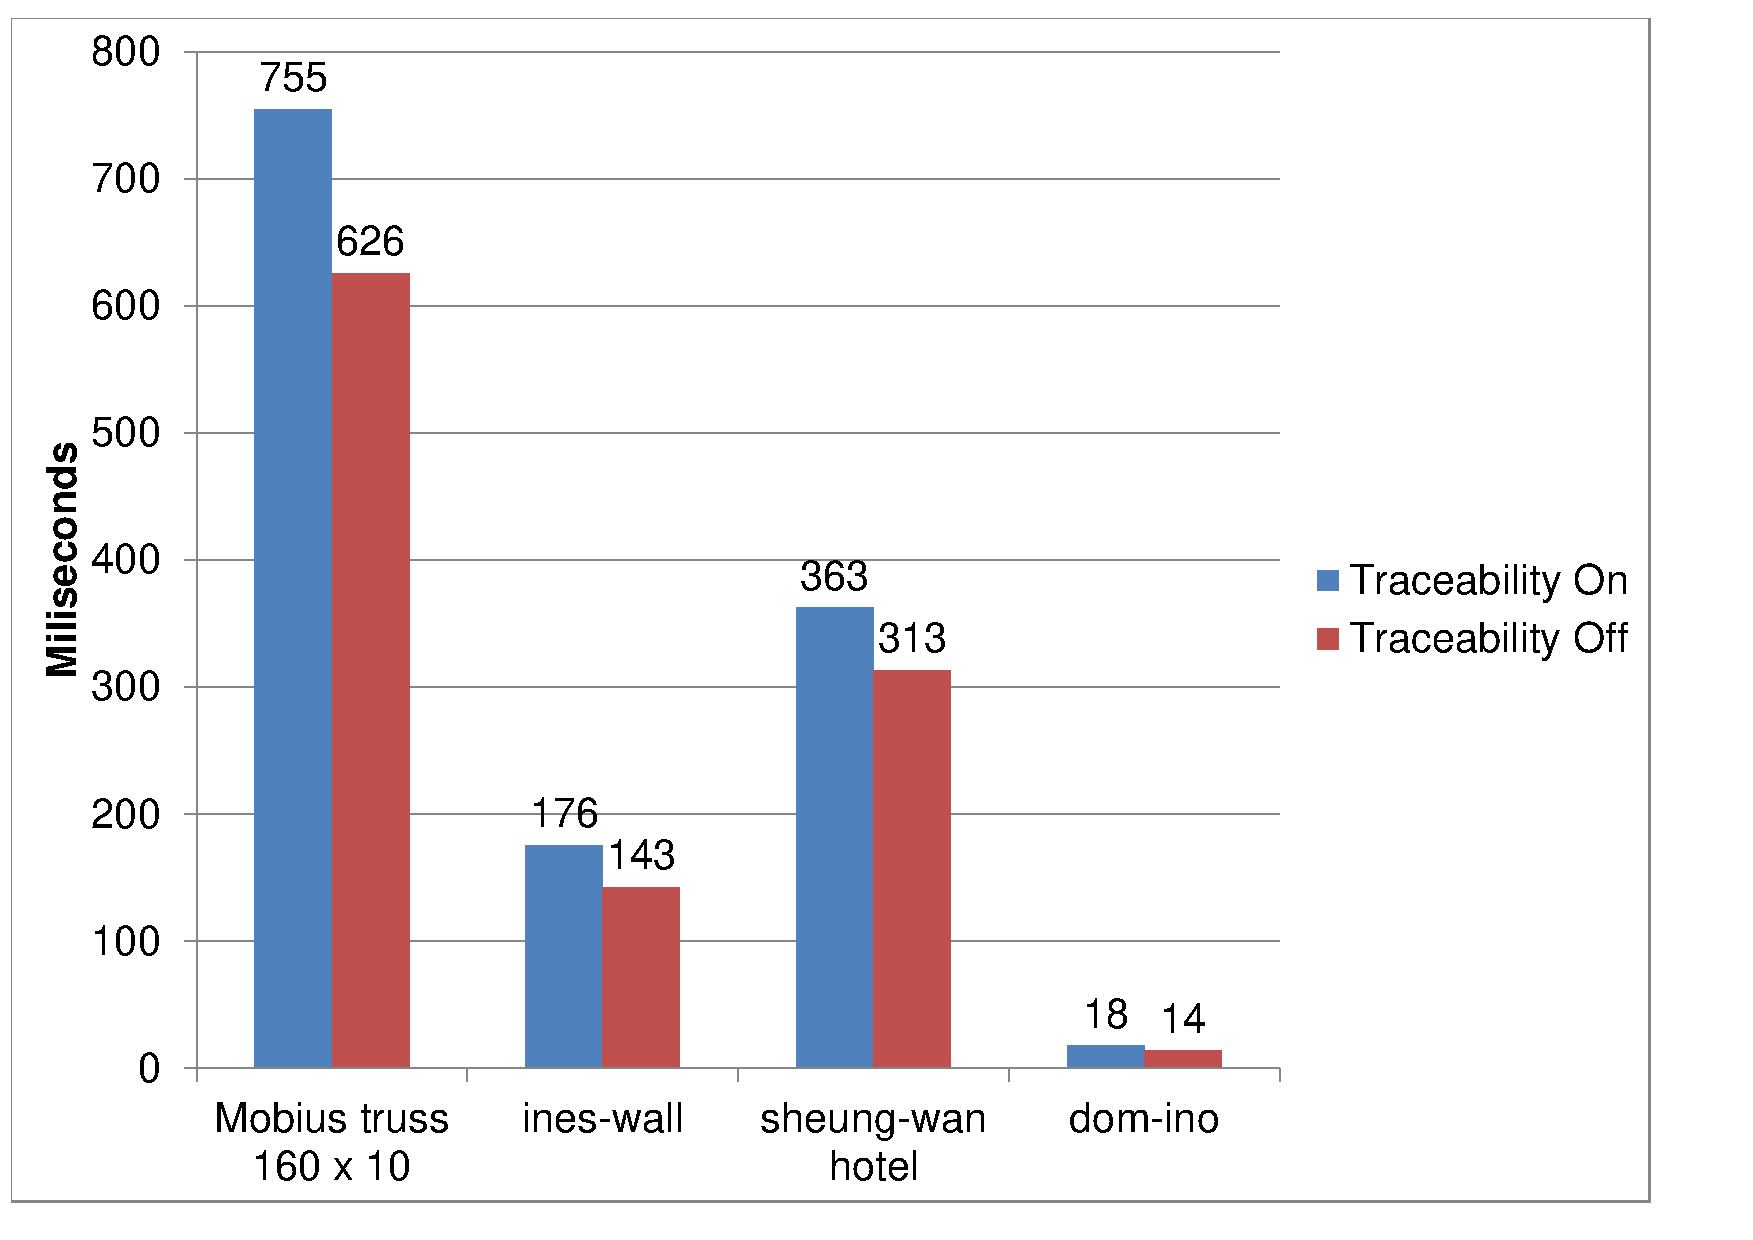
\includegraphics[width=12cm]{./images/traceability_timing}
  \caption{Running while collecting traceability data and while not collecting traceability data.}
  \label{fig:traceability:timing}
\end{figure}




%Describe possible programming techniques using the IDE / our solution.
%- Examples of use (made by me)
%- Example from architect (e.g. Inês Caetano)
%Describe possible use cases using our solution.

%GD capabilities(examples)
%- Architect example
%- More examples
%Performance:
%- web page vs rosetta vs grasshopper/dynamo
%- running in web page vs running in remote CAD service
%- impact of traceability tracking
%Geometry/primitives: our solution vs existing solutions

%Usefulness of traceability?
